\documentclass[11pt]{report}
\usepackage[utf8]{inputenc}
\usepackage[T1]{fontenc}
\usepackage{lmodern}
\usepackage[a4paper,margin=1in]{geometry}
\usepackage{amsmath,amssymb}
\usepackage{graphicx}
\usepackage{caption}
\usepackage[most]{tcolorbox}
\usepackage{microtype}
\usepackage{enumitem}
\usepackage{titlesec}
\usepackage{xcolor}
\usepackage[hidelinks]{hyperref}

\graphicspath{{figures/}}
\captionsetup{font=small,labelfont=bf,width=0.92\textwidth}
\setlength{\parskip}{4pt}
\setlength{\parindent}{0pt}

% ---- callout boxes (must match what the section writers use) ----
\definecolor{kibg}{HTML}{EAF3FB}\definecolor{kirule}{HTML}{2F6FB0}
\definecolor{anbg}{HTML}{FBF4E6}\definecolor{anrule}{HTML}{C0862A}
\definecolor{wlbg}{HTML}{ECF7EE}\definecolor{wlrule}{HTML}{3C8C53}

\newtcolorbox{keyidea}{colback=kibg,colframe=kirule,boxrule=0.8pt,arc=3pt,
  left=9pt,right=9pt,top=6pt,bottom=6pt,fonttitle=\bfseries,coltitle=white,
  colbacktitle=kirule,title=Key idea,breakable}
\newtcolorbox{analogy}{colback=anbg,colframe=anrule,boxrule=0.8pt,arc=3pt,
  left=9pt,right=9pt,top=6pt,bottom=6pt,fonttitle=\bfseries,coltitle=white,
  colbacktitle=anrule,title=Think of it like\ldots,breakable}
% tolerate an accidental optional argument from a writer, e.g. \begin{keyidea}[x]
\newcommand{\plainwords}[1]{\par\smallskip\noindent{\itshape In plain words.}~#1\par\smallskip}

\renewcommand{\thesection}{\arabic{section}}
\renewcommand{\thesubsection}{\thesection.\arabic{subsection}}
\titleformat{\section}{\normalfont\Large\bfseries\color{kirule}}{\thesection.}{0.6em}{}
\titlespacing*{\section}{0pt}{14pt}{6pt}

\begin{document}
\pagestyle{plain}

% ---- chapter front matter ----
\begin{center}
{\small\bfseries\color{kirule}\MakeUppercase{A chapter on safe AI for the physical world}}\\[10pt]
{\huge\bfseries Cool Heads}\\[6pt]
{\Large How a Digital Twin Saves Energy Without\\[2pt] Ever Overheating a Data Center}\\[14pt]
{\large Hoang-Huy Nguyen}\\[6pt]
\end{center}

\vspace{4pt}
\noindent\textit{Somewhere right now, a data center is being kept colder than it needs to be ---
burning electricity to buy peace of mind. This chapter is about a machine that learned to stop
doing that, safely: to run a server hall warmer and cheaper while promising, and proving week
after week, that it would never let a single computer breathe air that is too hot.}

\begin{tcolorbox}[colback=wlbg,colframe=wlrule,boxrule=0.8pt,arc=3pt,
  left=9pt,right=9pt,top=6pt,bottom=6pt,fonttitle=\bfseries,coltitle=white,
  colbacktitle=wlrule,title=What you'll learn]
\begin{itemize}[leftmargin=1.2em,nosep,itemsep=2pt]
  \item Why cooling a data center is a tug-of-war between saving energy and staying safe.
  \item What a ``digital twin'' is, and how planning inside a physics simulation beats guessing.
  \item The handful of equations that decide how cold to run a building --- each explained in plain words.
  \item How to let an optimizer get bolder \emph{only} as fast as it earns trust --- and never cross a safety line.
\end{itemize}
\end{tcolorbox}

\vspace{6pt}
\section{The thermostat dilemma}

Walk into a large data center and the first thing you notice is the cold. Aisles of humming servers, and yet the air feels like a supermarket freezer section. That chill is not an accident. It is a choice --- and an expensive one.

\begin{keyidea}
Data centers waste energy because the people running them cool too hard on purpose: over-cooling feels safe, but safety bought with brute-force refrigeration is paid for in electricity.
\end{keyidea}

To see why, picture the thermostat in your own home in the dead of summer. You could set it to a comfortable 24 degrees. But suppose you were terrified that one warm afternoon might ruin something priceless in the house --- and that the cost of that ruin would be catastrophic. What would you do? You would crank the dial down to 18, maybe lower, and leave it there all season. You would never be too hot. You would also pay a fortune, and most of that money would buy cold you never actually needed. That, in miniature, is the \emph{thermostat dilemma}: the cheapest way to feel safe is to over-cool, and over-cooling quietly burns money every minute of every day.

\begin{analogy}
A data center is a house full of priceless, heat-hating tenants --- the servers --- and the operator is the nervous homeowner with a hand on the thermostat, tempted to freeze the place just to be sure nothing ever overheats.
\end{analogy}

The stakes are higher than a home, because cooling is a genuinely big slice of a data center's total power bill. A useful way to talk about that slice is a single number called \emph{PUE}, short for Power Usage Effectiveness. The idea is simple: out of every watt the building draws from the grid, how much actually reaches the computers doing useful work, and how much is spent on everything else --- chiefly the cooling. We capture it like this.

\begin{equation}\label{eq:pue}
\mathrm{PUE} = \operatorname{mean}_t \left( \frac{P_{\text{total},t}}{P_{\text{IT},t}} \right)
\end{equation}
\plainwords{$P_{\text{total},t}$ is the total power the whole building pulls from the grid at moment $t$; $P_{\text{IT},t}$ is the slice of that going to the actual computing equipment (the ``IT'' load); the fraction is how many watts the building burns for every one watt of real computing, and $\operatorname{mean}_t$ just averages that ratio over time.}

A PUE of $1$ would be perfection: every single watt reaches the computers and nothing is lost to overhead. Reality is never that kind. If a building runs at a PUE of $2$, it burns one extra watt of cooling and overhead for every watt of computing --- effectively doubling the bill. The plan we will build in this chapter lands around $\mathrm{PUE} \approx 1.19$, meaning roughly $19$ cents of overhead on every dollar of computing. Shaving even a little off that number, across a building that runs every hour of every day, is real money and real carbon.

So why not just turn the cooling down and pocket the savings? Because the servers have a hard limit, and crossing it is not a ``pay a bit more'' problem --- it is a ``things break'' problem.

\begin{figure}[t]\centering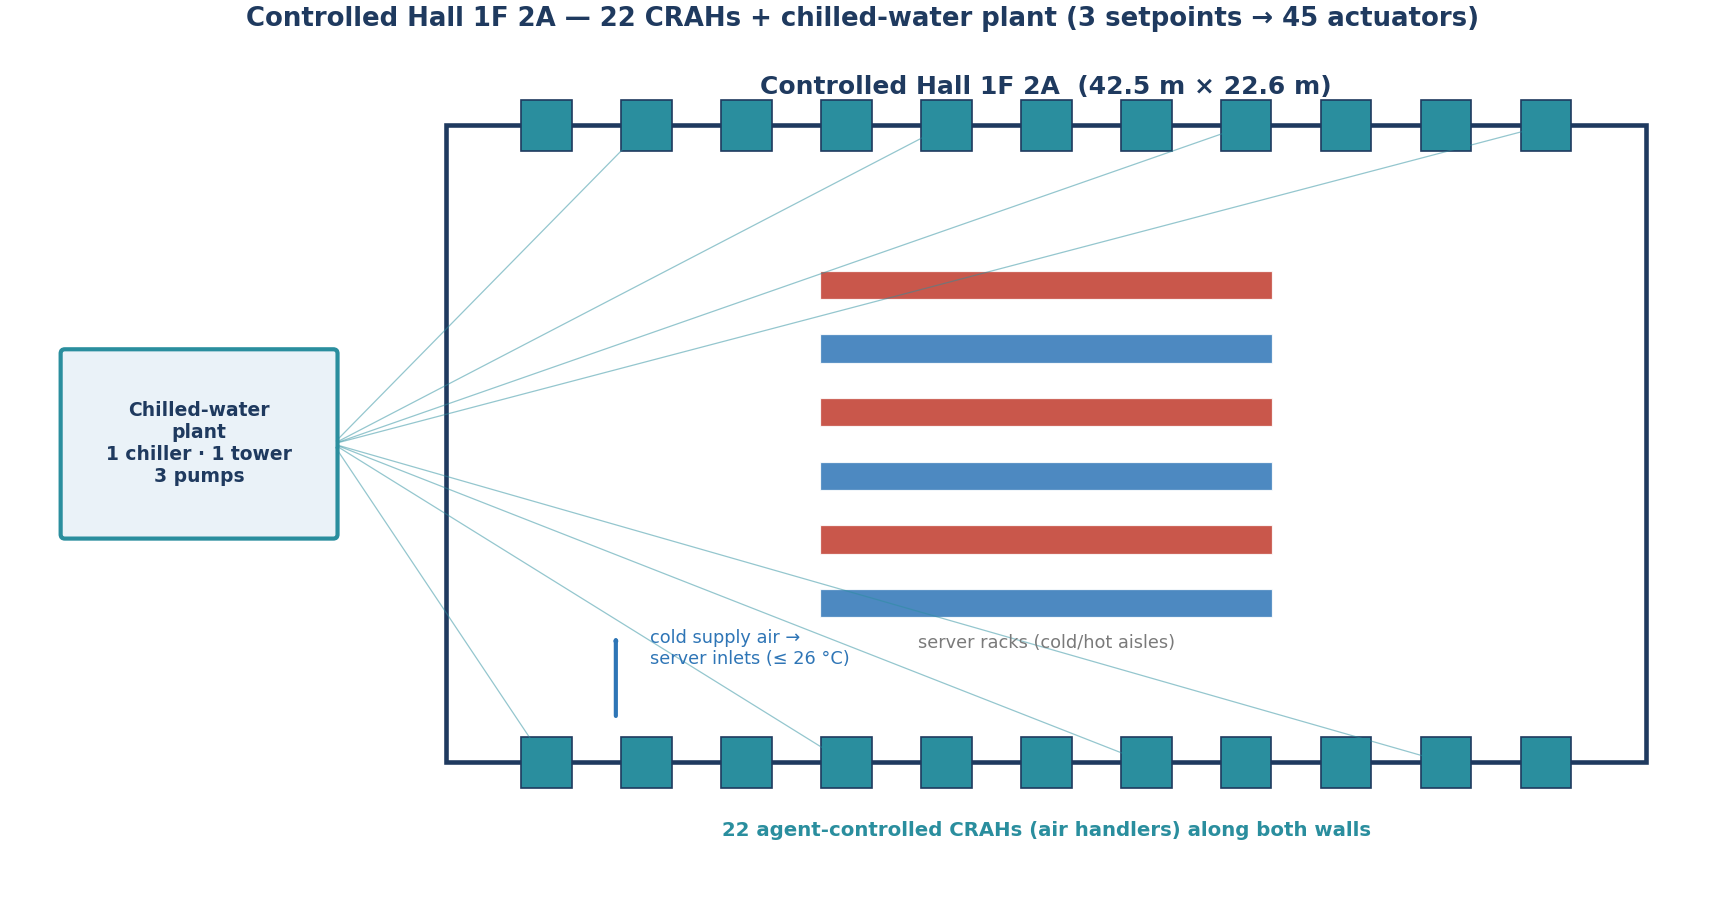
\includegraphics[width=0.85\linewidth]{figures/fig2_hall.png}\caption{The controlled hall: rows of server racks in hot/cold aisles, 22 air handlers, and a shared chilled-water plant. Three global dials are broadcast to 45 actuators that deliver cold air to the servers.}\label{fig:hall}\end{figure}

Figure~\ref{fig:hall} shows the room we are trying to tame: one hall of server racks, arranged so that cold air is blown in the front and hot exhaust streams out the back. Twenty-two air handlers push the cold air; a shared chilled-water plant makes the cold in the first place. Every server in that room breathes --- it pulls in air to carry away the heat it generates --- and the temperature of the air it breathes in is called the \emph{inlet temperature}, written $T_{\text{inlet}}$. If that intake air gets too hot, the chips inside cannot shed their heat fast enough, and they throttle, fault, or fail.

That gives us the one rule we are never allowed to break: every server's inlet air must stay at or below $26\,^\circ\mathrm{C}$, at every fifteen-minute step, forever. Not ``on average.'' Not ``almost always.'' The $26\,^\circ\mathrm{C}$ cap is a hard ceiling, the equivalent of the homeowner's vow that the priceless tenants must never, ever get too warm.

\begin{keyidea}
The whole problem is a tug-of-war between two forces pulling in opposite directions: spend less energy on cooling, versus never let any server breathe air hotter than $26\,^\circ\mathrm{C}$.
\end{keyidea}

This is what makes the dilemma genuinely hard rather than merely annoying. The two goals fight each other. Pushing the cooling down to save energy nudges every inlet temperature \emph{up}, closer to the cliff edge of the cap. The timid answer --- the one most operators reach for --- is to keep a huge safety buffer, run the room far colder than it needs to be, and accept the waste as the price of a good night's sleep. The ambitious answer is to creep right up to the edge of the cap and hold there: as warm as is safe, and not one degree warmer. But creeping up to a cliff edge in a building full of priceless tenants is exactly the kind of thing nobody wants to do by trial and error on the real plant. We need somewhere safe to practice.

\section{A flight simulator for a data center}

Pilots do not learn to handle an engine fire by setting their actual engine on fire. They climb into a flight simulator --- a faithful computer model of the real aircraft --- and try the terrifying maneuver there, as many times as they like, where a mistake costs nothing. Only once they have found a move that works do they take it to the real cockpit. We are going to do exactly the same thing for a data center.

\begin{keyidea}
Build a faithful physics simulation of the hall --- a ``digital twin'' --- try every risky cooling decision inside it first, and only carry the winning, proven-safe decision out to the real building.
\end{keyidea}

\begin{analogy}
The digital twin is a flight simulator for the building. We rehearse the scary moves --- running the room warmer to save energy --- in the simulator, where overheating a virtual server costs nothing, and we only fly the real plane once we have a plan that lands safely.
\end{analogy}

A \emph{digital twin} is just that flight simulator. In our case it is a full-physics building simulation --- we use a mature, industry-standard engine called EnergyPlus (version 9.5), running inside a Docker container so it behaves identically every time --- that takes a proposed set of cooling settings and a week of expected weather and computing load, and plays the whole week forward in fifteen-minute steps. Out the other end it tells us two things we care about above all: how much cooling energy that plan would burn, and whether any server's inlet would ever breach the $26\,^\circ\mathrm{C}$ cap. Because it is ``in the loop'' --- consulted on every candidate decision --- we call it the \emph{oracle}: the judge that scores each plan before anyone touches the real plant.

Once a week, the system reaches for three ``dials'' --- three global setpoints that govern the whole hall. The first is the supply-air temperature, $T_{\text{supply}}$: how cold the air being blown in actually is, allowed to range from $20$ to $26\,^\circ\mathrm{C}$. The second is the airflow: how hard the air handlers blow, from $4.8$ to $13.8$ kilograms of air per second per unit. The third is the chilled-water supply temperature, CHWST, the temperature of the water the plant chills to make all that cold air, from $13$ to $19\,^\circ\mathrm{C}$. Just three numbers --- but the system fans them out to $45$ individual actuators across the room, and together they decide both the energy bill and every server's fate.

\begin{figure}[t]\centering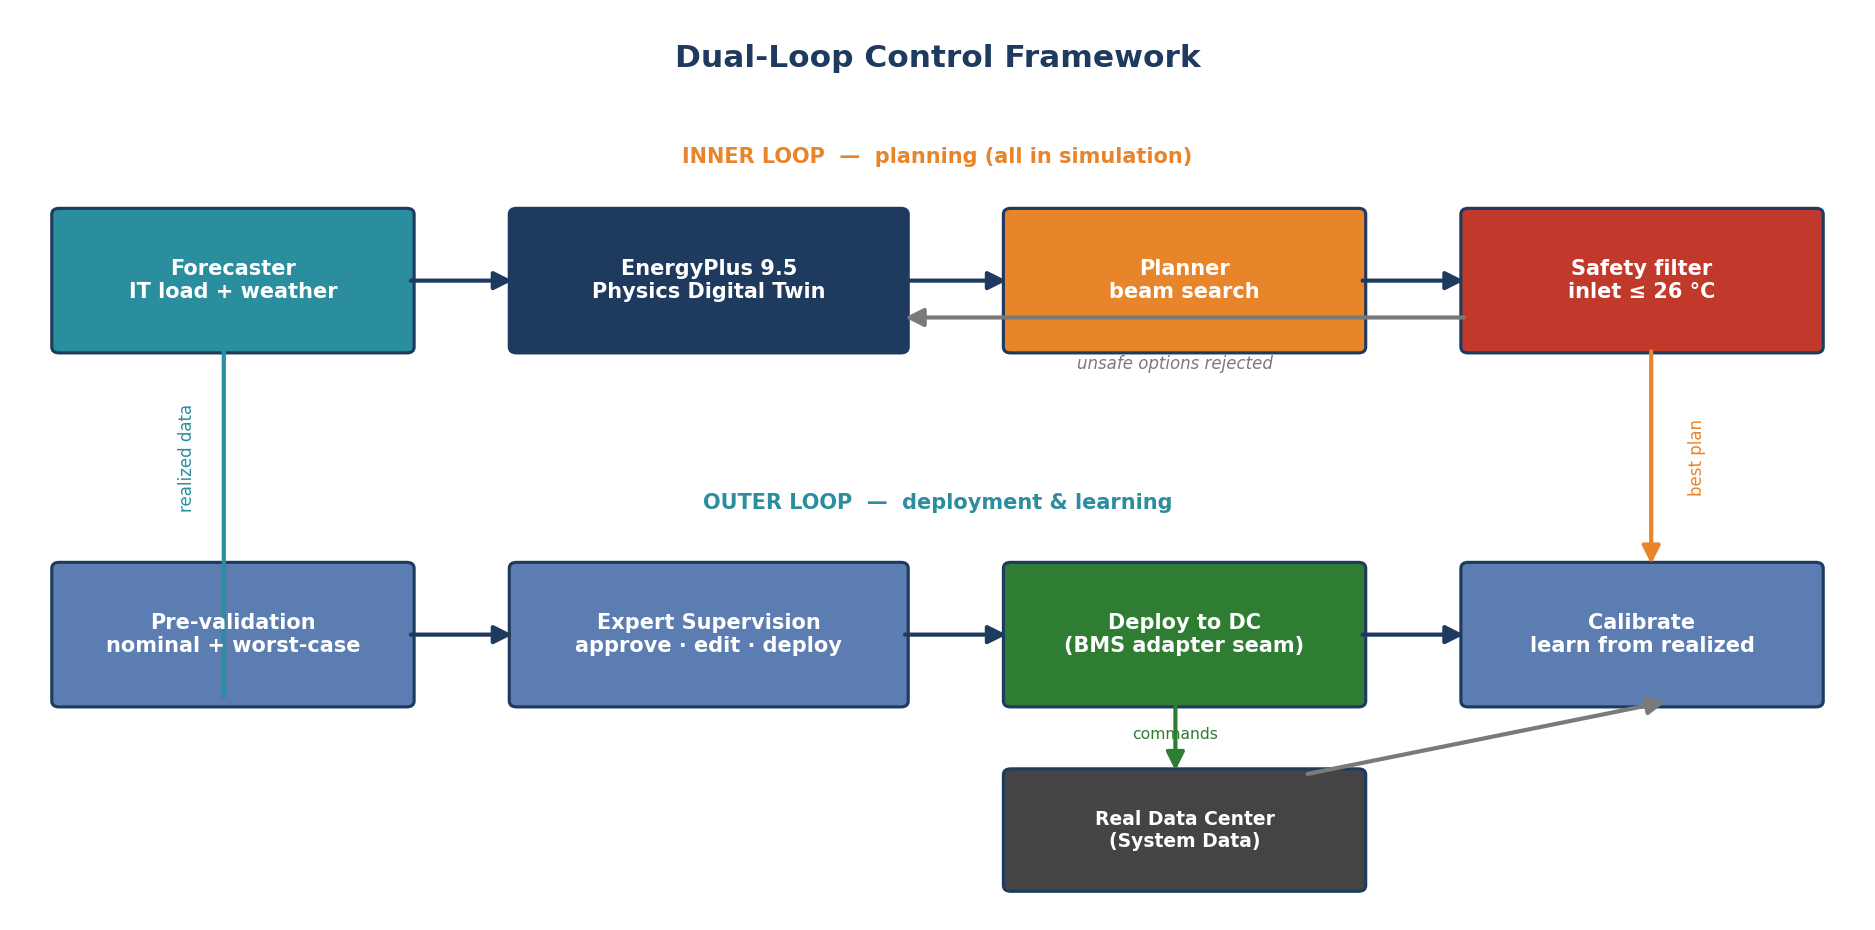
\includegraphics[width=\linewidth]{figures/fig3_arch.png}\caption{The dual loop. \emph{Inner loop}: a forecaster feeds a search that proposes setpoints, each scored by a full-week physics simulation, with unsafe options filtered out. \emph{Outer loop}: the chosen plan is pre-validated, an expert approves it, it is deployed, and the measured result teaches the next week's plan.}\label{fig:arch}\end{figure}

The way these pieces fit together is the heart of the whole framework, and it is built as two nested loops --- a \emph{dual loop}. Figure~\ref{fig:arch} lays it out.

The \emph{inner loop} all happens inside the simulator, where nothing can be harmed. It starts with a forecaster that guesses the coming week's weather and computing load. A search then proposes candidate settings for the three dials, and hands each candidate to the digital-twin oracle, which plays the full week forward and scores it. Crucially, any candidate that would ever overheat a server is thrown out before it can win --- unsafe options simply never make it onto the shortlist. The inner loop's job is to find the cheapest plan that is also safe, and to do all of that thinking in simulation.

The \emph{outer loop} is where we cautiously touch reality. The plan the inner loop chose is first put through a pre-validation gate, then shown to a human expert who approves it, and only then is it deployed to the hall. Afterward --- and this is the part that makes the system get smarter over time --- we measure what actually happened and compare it to what the twin predicted. Any gap between prediction and reality is fed back to sharpen the twin, so next week's plan starts from a more honest model of the building. The inner loop optimizes; the outer loop deploys carefully and learns. That is the dual loop.

\begin{keyidea}
Inner loop: plan boldly but only inside the simulator. Outer loop: act cautiously in reality, then learn from the difference between what was predicted and what happened.
\end{keyidea}

That is the whole idea in one breath. The rest of this chapter unpacks it piece by piece, in the order the system itself works: first the three \emph{dials} and how they move the room; then the \emph{physics} that turns cold air into safe (or unsafe) servers; then the \emph{search} that hunts for the cheapest safe plan; then the layered \emph{safety} nets that guarantee we never cross the $26\,^\circ\mathrm{C}$ cap; then the \emph{learning} that closes the loop week after week; and finally the \emph{results} from six consecutive deployed weeks. Keep the two anchors in mind the whole way --- the thermostat dilemma we are trying to escape, and the flight simulator we use to escape it safely.

\section{Three dials and forty-five hands}

\begin{keyidea}
A whole data-center hall is cooled by turning just three master dials --- how cold the air is, how hard it is blown, and how cold the chilled water is --- and each tiny turn of a dial ripples out to forty-five separate hands tweaking the actual equipment.
\end{keyidea}

Imagine standing in front of a giant cooling machine the size of a warehouse and being told you may touch only three knobs. That is, in essence, DCTwin's job. The hall we control is called ``1F 2A''. Inside it sit racks of computers drawing about 2.0 megawatts of power --- roughly the electricity of two thousand homes --- and every watt that goes in comes back out as heat. Twenty-two air handlers, called CRAH units (Computer Room Air Handlers), fight that heat by pushing cold air through the room. All of them, plus the shared chilled-water plant, answer to just three commands.

Here is what each dial does, in plain physical terms.

The first dial is the \emph{supply-air temperature}, $T_{\text{supply}}$ --- how cold the air leaving the air handlers is. It can be set anywhere from $20$ to $26\,^\circ$C. Colder air sounds safer, and it is, but making air colder costs energy, like running your home air conditioner at full blast. This is the heart of the thermostat dilemma: the timid instinct is to set the air very cold ``just to be safe,'' and that timidity is exactly what wastes money.

\begin{analogy}
Setting the supply-air temperature is like choosing how cold to make the air coming out of your car's vents. Crank it to maximum cold and you are comfortable but burning fuel; ease off and you save fuel but flirt with getting too warm.
\end{analogy}

The second dial is the \emph{airflow} --- how much air each CRAH blows, measured in kilograms of air per second, allowed to range from $4.8$ to $13.8$ kg/s per unit. This is the strength of the fan. More airflow carries heat away faster, but fans themselves guzzle power, and a fan's appetite grows steeply as you speed it up. Blow too little air, though, and something sneaky happens that we will return to in the next section: the hot exhaust starts sneaking back to the front of the servers.

The third dial is the \emph{chilled-water supply temperature}, CHWST --- how cold the water is that the plant sends to the air handlers' cooling coils, allowed to range from $13$ to $19\,^\circ$C. Colder water cools the air more aggressively but forces the chiller to work harder. Warmer water lets the chiller relax and sip less power, which is often where the easy savings hide.

So we have three dials: $T_{\text{supply}}$ ($20$--$26\,^\circ$C), airflow ($4.8$--$13.8$ kg/s), and CHWST ($13$--$19\,^\circ$C). But the hall does not have three controls --- it has forty-five. There are 22 individual supply-temperature settings (one per air handler), 22 individual airflow settings, and 1 chilled-water-plant setting, for a total of $22 + 22 + 1 = 45$ separate actuators, each a real ``hand'' on a real piece of equipment.

DCTwin bridges this gap by \emph{broadcasting}: it reasons about the three global dials, then copies each setting out to all the matching actuators at once. The three numbers it chooses fan out into forty-five commands. This keeps the decision small enough to think about clearly --- searching over three dials, not forty-five --- while still steering every machine in the room.

\section{Asking the laws of physics}
\label{sec:oracle}

\begin{keyidea}
Before DCTwin trusts any cooling plan, it does not guess what will happen --- it runs the entire week through a full-physics simulation of the building, so every plan is judged by the laws of physics rather than by hope.
\end{keyidea}

Here is the trap inside the thermostat dilemma: the safe-feeling move (more cold, more air) and the cheap move (less cold, less air) pull in opposite directions, and the consequences are not obvious. Turn a dial and the effect ripples through twenty-two air handlers, a chilled-water plant, two megawatts of heat, and the messy way air actually swirls around a room. A back-of-the-envelope guess will not capture that. So DCTwin does something more honest: it asks the laws of physics directly, through the flight simulator we met earlier --- the EnergyPlus oracle.

For any candidate plan, the oracle plays out a full week of the building's behaviour in fifteen-minute steps and reports back exactly how much energy was used and how hot every server got. It is slow, but it does not lie. Let us see what it reports, one quantity at a time.

\subsection*{Counting the energy, step by step}

The first thing the oracle reports is energy. At each fifteen-minute step the cooling system draws some electrical power, and power held for a stretch of time is energy. So for each step we multiply the cooling power by the length of the step.

\begin{equation}\label{eq:energy-step}
E_t = \frac{P_{\text{hvac},t} \cdot \Delta t}{1000} \quad \text{(kWh)}, \qquad \Delta t = 0.25\ \text{h}.
\end{equation}
\plainwords{$E_t$ is the energy used in one time step (in kilowatt-hours). $P_{\text{hvac},t}$ is the cooling power --- the fans plus the chiller and chilled-water plant --- measured in watts during that step. $\Delta t$ is how long the step lasts, which is $0.25$ hours, i.e. fifteen minutes. Dividing by $1000$ just converts watts into kilowatts so the answer lands in the familiar kilowatt-hour unit on your electricity bill.}

A week has many such steps, so the weekly cooling energy is simply all of them added up.

\begin{equation}\label{eq:energy-week}
E_{\text{hvac}} = \sum_{t} E_t.
\end{equation}
\plainwords{$E_{\text{hvac}}$ is the total cooling energy for the whole week. The symbol $\sum_t$ means ``add up over every fifteen-minute step $t$ in the week.'' It is the running total on the meter once the simulated week is over.}

The same simulation also tracks the building's overall efficiency through the PUE of Equation~\ref{eq:pue} --- the ratio of total facility power to computing power that we met at the very start. DCTwin's chosen plan runs the hall at about $\mathrm{PUE} \approx 1.19$: roughly nineteen cents of cooling-and-overhead for every dollar of real computing.

\subsection*{Why the temperature you set is not the temperature a server breathes}

Now the subtle part --- and the reason a guess is so dangerous. You set the supply air to, say, $22\,^\circ$C. You might assume every server therefore breathes $22\,^\circ$C air. It does not. Some of the hot air a server just exhaled curls around and gets sucked back into its own intake before the cold air reaches it. The air a server actually breathes is a \emph{mixture} of fresh cold supply air and leaked-back hot exhaust.

\begin{equation}\label{eq:inlet-mixing}
T_{\text{inlet}} = r\,T_{\text{return}} + (1-r)\,T_{\text{supply}}.
\end{equation}
\plainwords{$T_{\text{inlet}}$ is the temperature of the air a server actually draws in. $T_{\text{supply}}$ is the cold air you sent. $T_{\text{return}}$ is the warm exhaust air on its way back to the air handler. $r$ is the \emph{recirculation fraction} --- a number between $0$ and $1$ saying what share of the inlet air is leaked-back hot exhaust rather than fresh cold air. If $r=0$, no leak: the server breathes exactly the supply temperature. If $r=0.3$, three-tenths of what it breathes is hot return air, so its intake is warmer than you ever set the dial. This gap is precisely why the temperature you set is not the temperature a server breathes.}

Because the safety limit is on what the servers breathe, this mixing is everything. We can even turn the formula around to measure the leak from observed temperatures.

\begin{equation}\label{eq:recirc-solve}
r = \frac{T_{\text{inlet}} - T_{\text{supply}}}{T_{\text{return}} - T_{\text{supply}}}.
\end{equation}
\plainwords{This is just Equation~\ref{eq:inlet-mixing} rearranged to solve for the leak fraction $r$. In words: take how much hotter the inlet is than the supply air, and divide by how much hotter the return air is than the supply air. The bigger that ratio, the more hot exhaust is sneaking back into the servers' faces.}

\subsection*{Starve the fans and the inlets get hotter}

Here is where the airflow dial bites back. If you blow less air than the room actually needs to clear its heat, the cold air no longer reaches every server cleanly, and recirculation gets worse. The oracle models this with a flow-shortfall rule.

\begin{equation}\label{eq:recirc-flow}
r_{\text{eff}} = \min\!\left(0.5,\; r_0 + 0.5 \cdot \max\!\left(0,\; 1 - \frac{\text{flow}}{\text{demand}}\right)\right).
\end{equation}
\plainwords{$r_{\text{eff}}$ is the effective recirculation fraction once we account for weak airflow. $r_0$ is the baseline leak you would get with plenty of air. ``flow'' is how much air you are actually blowing; ``demand'' is how much the room needs. The fraction $\text{flow}/\text{demand}$ is $1$ when you supply exactly enough air. The term $\max(0,\,1 - \text{flow}/\text{demand})$ is the \emph{shortfall}: zero if you have enough air, and growing the more you fall short. That shortfall, scaled by $0.5$, adds to the leak. The outer $\min(0.5,\dots)$ caps the leak at one half --- even a badly starved room never breathes more than $50\%$ recirculated air in this model.}

Put Equations~\ref{eq:inlet-mixing} and~\ref{eq:recirc-flow} together and the danger is plain: skimping on airflow to save fan power raises $r_{\text{eff}}$, which through the mixing identity raises $T_{\text{inlet}}$ --- pushing the servers' intake air closer to the hard $26\,^\circ$C cap. The cheapest-looking move is also the most likely to overheat a server. That is the thermostat dilemma in equation form, and it is exactly why DCTwin will not accept a plan on a hunch. It makes the flight simulator play out the whole week first, watching every inlet at every fifteen-minute step, before a single real dial is touched.

\section{Searching for the sweet spot}
\label{sec:search}

\begin{keyidea}
The planner does not guess a single answer; it scans the whole space of possible cooling settings coarsely, zooms in on the most promising regions, and scores each candidate with one number --- but a setting that would ever cook a server is given an infinite score, so it can never win.
\end{keyidea}

Recall the thermostat dilemma: turn the cooling up and you are safe but wasteful; turn it down and you save money but flirt with overheating. Somewhere between those extremes lies a sweet spot --- the cheapest setting that is still provably safe. The trouble is that we have three dials to turn at once (the supply-air temperature $T_{\text{supply}}$, the airflow, and the chilled-water temperature CHWST), and every combination behaves differently. How do you find the best corner of a three-dimensional room when you cannot afford to stand in every spot?

\begin{analogy}
Imagine searching a vast hilly map for the lowest point in a valley. You do not measure the altitude at every square metre --- that would take forever. Instead you drop a coarse grid of survey stakes across the whole map, find the handful of stakes that sit lowest, and then plant a finer grid of stakes around just those promising spots. Repeat, tightening the net each time, and you close in on the bottom of the valley without ever surveying the whole landscape.
\end{analogy}

\subsection{Scoring a setting: one number, lower is better}

Before we can search, we need a way to rank any candidate setting. We boil everything down to a single score $J$ --- think of it as the ``bill'' for running the week, where a smaller bill is better. The bill is mostly the cooling energy, plus a few gentle surcharges for letting conditions drift out of their comfortable bands.

\begin{equation}
\label{eq:objective}
J = E^{*} + 1.0\,S_{\text{inlet}} + 0.2\,S_{\text{rh}} + 0.1\,S_{\text{zone}}.
\end{equation}
\plainwords{$J$ is the overall score we want to make as small as possible (lower is better). $E^{*}$ is the week's cooling energy $E_{\text{hvac}}$ (or, if we are pricing electricity, the tariff-weighted cost of that energy) --- the main part of the bill. $S_{\text{inlet}}$ is a ``drift penalty'' that piles up whenever server intake temperatures wander toward the edge of their comfortable range; $S_{\text{rh}}$ does the same for humidity (``rh'' = relative humidity); $S_{\text{zone}}$ for the room's air temperature. The numbers $1.0$, $0.2$, $0.1$ are weights that say how much each kind of drift adds to the bill: inlet drift is taken most seriously, humidity less so, zone temperature least.}

These three penalties are soft nudges, not hard rules. They gently steer the search away from settings that are technically allowed but uncomfortable --- like a thermostat that lets the room get a little muggy. The real wall, the line that must never be crossed, is handled separately and far more bluntly.

\begin{keyidea}
A candidate that would ever push a server's inlet above the $26\,^\circ$C cap is not merely penalised --- it is disqualified. We set its score to $J = +\infty$, so no amount of energy saving can ever let an unsafe setting win.
\end{keyidea}

This is the planner's version of the flight simulator. We let it ``fly'' every candidate setting through a full simulated week (the EnergyPlus oracle of Section~\ref{sec:oracle} does the flying). If the simulated flight ever shows a server breathing air hotter than $26\,^\circ$C, the candidate crashes the plane --- and a crashed plane scores infinitely badly. The search therefore minimises $J$ over the \emph{safe} candidates only; everything unsafe is invisible to it.

\subsection{Coarse-to-fine beam search}

Now to the searching itself. The planner uses a method called \emph{beam search}, which is exactly the survey-stakes strategy from our map analogy, made precise.

\paragraph{Step 1 --- the coarse grid.} It starts by laying down a coarse grid across the whole space of the three dials: five evenly spaced values for the supply-air temperature, five for the airflow, and five for the chilled-water temperature. Every combination is one candidate, which gives $5 \times 5 \times 5 = 125$ settings to try. Each of these 125 is flown through its simulated week and scored with $J$.

\paragraph{Step 2 --- keep the best 5.} Out of those 125 survey stakes, the planner keeps only the five with the lowest scores --- the five most promising corners of the room. This shortlist is the ``beam'' that gives the method its name: instead of carrying every possibility forward, we keep a narrow beam of the best few.

\paragraph{Step 3 --- zoom in, three times.} Around each of those five survivors, the planner plants a finer grid of nearby candidates, scores them, and again keeps the best five overall. Crucially, the spacing of the grid is \emph{halved} at every level: the stakes get twice as close together each time, so the search zooms in on the sweet spot with ever-finer resolution. It repeats this refine-and-shortlist cycle for three levels of zoom.

\paragraph{Step 4 --- stop when it stops helping.} There is no point grinding on once the improvements have shrunk to nothing. So the search watches how much the best score drops from one level to the next; if it improves by less than a tiny threshold ($\epsilon = 10^{-3}$), it stops early. We have effectively reached the bottom of the valley, and digging further wins nothing.

The payoff of this coarse-to-fine approach is efficiency: each simulated week is expensive (it is a full physics run), so we cannot afford to score thousands of settings. By scanning coarsely first and spending the fine-grained effort only where it matters, the planner finds a near-optimal setting with a few hundred simulated weeks instead of a brute-force sweep of the entire space.

\subsection{Why this is a real problem: energy and safety pull apart}

It would be tempting to think the answer is obvious --- just turn everything down to save the most energy. Figure~\ref{fig:wellposed} shows why that instinct is dangerous, and why a hard-constrained search is genuinely needed rather than a simple ``minimise energy'' rule.

\begin{figure}[t]\centering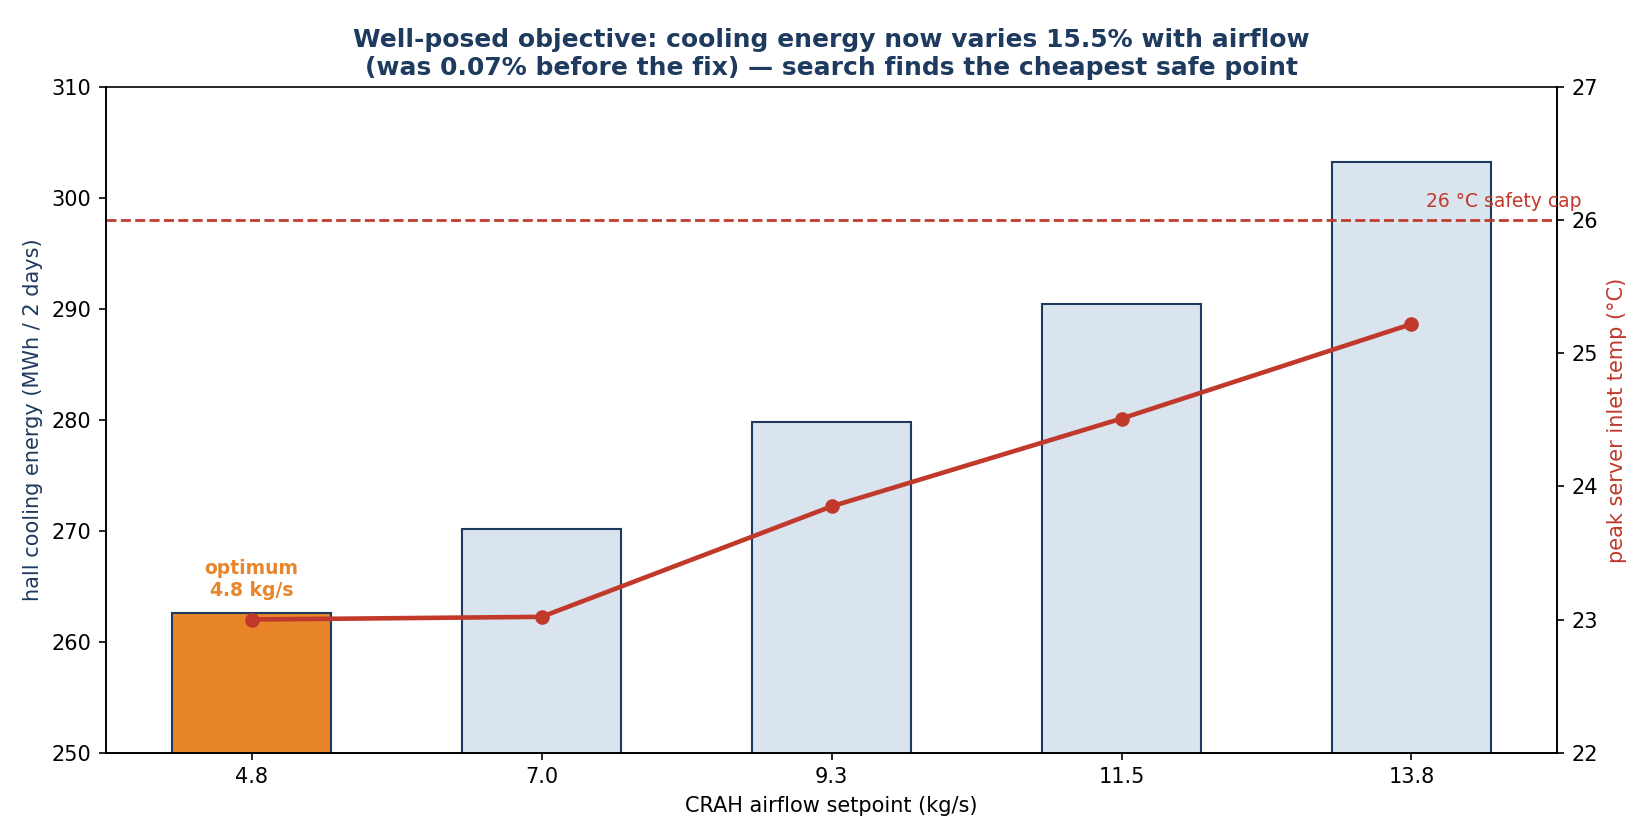
\includegraphics[width=0.85\linewidth]{figures/fig4_results.png}\caption{Why the problem is real. As airflow changes, cooling energy swings by about 15.5\% (bars) while the hottest server inlet (line) climbs toward the 26\,$^\circ$C cap. The cheapest setting is also the hottest --- so you cannot just minimise energy; you must respect the line.}\label{fig:wellposed}\end{figure}

The figure comes from a controlled sweep on the real EnergyPlus physics, turning each dial in turn to see how much it moves the hall's cooling energy. Airflow is by far the strongest lever: dialling it changes cooling energy by about $15.5\%$. (For comparison, the chilled-water temperature moves energy by about $3.4\%$ and the supply-air temperature by only about $0.5\%$.) So if all you cared about was the bill, you would cut the airflow to the bone.

But look at the line in the figure. The very setting that uses the least energy --- the lowest airflow --- is also the one that drives the hottest server inlets up toward the $26\,^\circ$C cap. Less air moving through the hall means more hot exhaust recirculates back into the cold aisle (the flow-shortfall effect of Equation~\ref{eq:recirc-flow}), and intake temperatures climb. Energy and safety are pulling in opposite directions: the cheapest corner of the room is also the most dangerous one.

That tension is the whole reason the search must be \emph{constrained} rather than merely \emph{minimised}. A naive optimiser chasing the lowest energy would march straight to the hottest, most fragile setting and declare victory. DCTwin instead minimises the bill $J$ only among settings that stay provably on the safe side of the line --- which is precisely what the $J = +\infty$ disqualification, and the safety nets of the next section, are there to guarantee.

\section{Never crossing the line}

\begin{keyidea}
Safety is a wall, not a wish. The energy bill is something DCTwin tries to lower; the $26\,^\circ$C inlet limit is something it is forbidden to cross. The whole design exists so that one good week of cooling can never tempt the system into one bad minute.
\end{keyidea}

Recall the thermostat dilemma. A nervous operator over-cools the hall to be safe, and burns money doing it. DCTwin is supposed to walk much closer to the edge --- to let the servers run a little warmer and pocket the savings. But walking closer to a cliff is only wise if you are very sure where the cliff is. The danger is obvious: a plan that looks cheap on paper might, on a hot afternoon or with a tired chiller, push some server's intake air past $26\,^\circ$C. That is the line we must never cross.

So DCTwin does not trust a single calculation. It stacks \emph{three independent safety nets}, each one guarding against a different way the first net could be fooled. If the first net's estimate is slightly wrong, the second catches it; if the second is somehow optimistic, the third catches it after the fact. Figure~\ref{fig:safety} shows the three nets stacked, and the bottom line they produced: across six deployed weeks the hottest inlet ever recorded was $25.60\,^\circ$C, and the line was never crossed.

\begin{figure}[t]\centering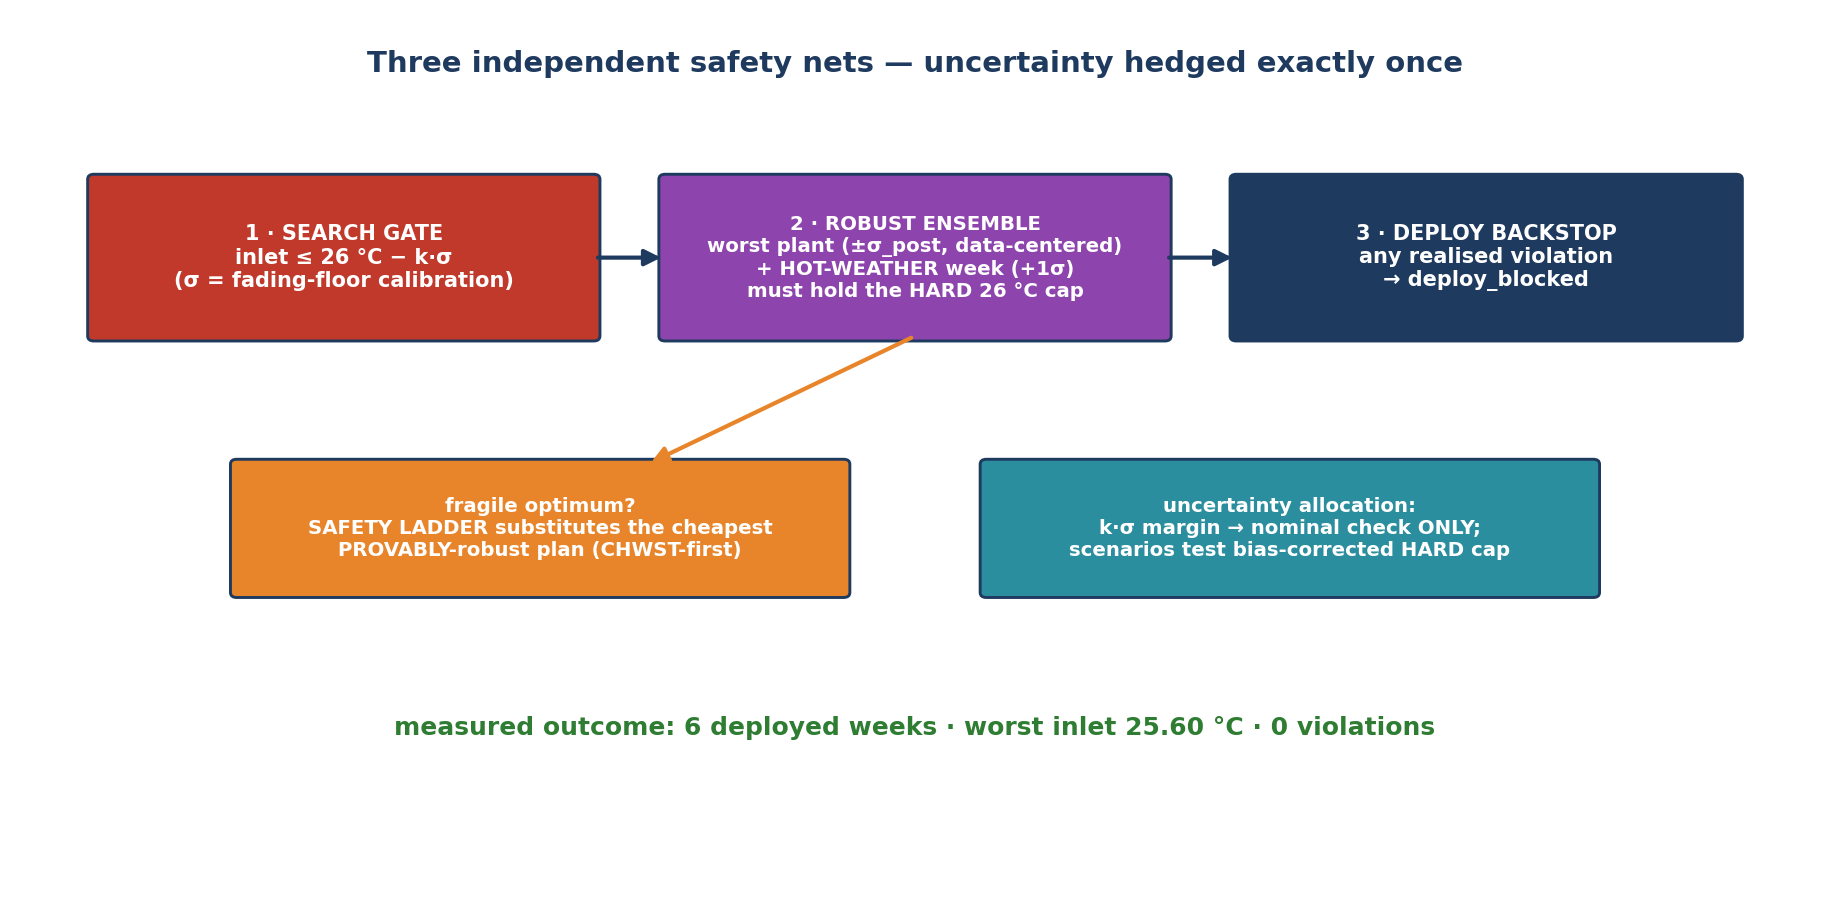
\includegraphics[width=\linewidth]{figures/figD_safety_stack.png}\caption{Three independent safety nets: a margin baked into the search, a worst-case stress-test ensemble, and a zero-tolerance backstop after the fact. Measured outcome: worst inlet 25.60\,$^\circ$C, zero violations.}\label{fig:safety}\end{figure}

\subsection{Net 1 --- a safety margin you can't argue with}

\begin{keyidea}
The first net refuses to aim for the line itself. It aims for a target safely below the line, and the size of that safety gap grows with how unsure the twin is about its own prediction.
\end{keyidea}

\begin{analogy}
Think of a hiker on a cliff path who knows their GPS can be off by a few steps. They don't walk where the GPS says the edge is --- they stay back by at least the GPS's margin of error. If the GPS is shaky today, they stay back further. DCTwin does exactly this with temperature.
\end{analogy}

When DCTwin scores a candidate plan inside the flight simulator, it doesn't just check ``did any inlet go over $26\,^\circ$C in the simulation?'' That would be trusting the simulation perfectly. Instead it demands two things at once: zero steps over the cap \emph{and} that the predicted peak inlet, plus a safety margin, still sits under $26\,^\circ$C. The margin is set by how unsure the twin is.

\begin{equation}\label{eq:margin}
m = k \cdot \sigma, \qquad k = 1.
\end{equation}
\plainwords{$m$ is the safety gap, in degrees Celsius, that we insist on keeping below the $26\,^\circ$C limit. $\sigma$ (``sigma'') is the twin's own honest estimate of how unsure it is about its inlet-temperature prediction --- a small $\sigma$ means ``I'm confident,'' a large $\sigma$ means ``I might be off by this much.'' $k$ is a dial for how cautious to be; we set $k=1$, meaning ``stay back by one full unit of your own uncertainty.''}

A candidate plan is allowed through the first net only if it satisfies the feasibility test below.

\begin{equation}\label{eq:feasible}
\text{(steps over cap)} = 0 \quad\text{and}\quad T_{\text{inlet}}^{\text{peak}} + m \;\le\; 26\,^{\circ}\text{C}.
\end{equation}
\plainwords{The plan must have zero moments where any server's intake air went over the limit, \emph{and} its hottest predicted intake temperature ($T_{\text{inlet}}^{\text{peak}}$) plus the safety gap $m$ must still fit under $26\,^\circ$C. If either test fails, the plan is rejected before it can even compete on price.}

Here is the elegant part: the safety gap is not a fixed fudge factor someone guessed. It \emph{breathes} with the twin's confidence. When DCTwin is brand new and has never been tested against reality --- a ``cold start'' --- it sensibly assumes it might be wrong by a whole degree, so $\sigma = 1.0\,^{\circ}$C. With $k=1$, the margin is $m = 1.0\,^{\circ}$C, and the search effectively treats the real limit as $25.0\,^{\circ}$C, not $26.0$. A fresh, untested twin is forced to be timid. Later, after the twin has proven itself accurate week after week, $\sigma$ shrinks and the margin shrinks with it, so the search is allowed to walk a little closer to the line and harvest more savings --- but only because it has \emph{earned} the right to.

\subsection{Net 2 --- the stress test: judge a plan by its bad days}

\begin{keyidea}
The second net doesn't ask ``is this plan fine on a normal day?'' It asks ``is this plan still fine if the equipment is worse than we think and the weather is hotter than forecast?'' A plan is only trusted if it survives the rough scenarios, not just the average one.
\end{keyidea}

The first net guards against the twin being a little uncertain. But what if the world itself misbehaves --- a chiller that's losing efficiency, a fan that under-delivers, a week that runs hotter than the forecast said? The second net handles this by taking the handful of finalist plans and re-running each one inside a small \emph{ensemble} of pessimistic, ``what if the plant is worse'' versions of the simulator, plus a deliberately hot week (the forecast nudged up by one unit of weather uncertainty, $+1\sigma$).

How wide should ``pessimistic'' be? Again, it adapts to how much the twin has learned.

\begin{equation}\label{eq:ensemble}
s = \min\!\Big(0.10,\ \max\big(0.02,\ 0.10\cdot \tfrac{\sigma_{\text{post}}}{1.0}\big)\Big).
\end{equation}
\plainwords{$s$ is the half-width of the stress test --- how far in each direction we knock the plant ``worse,'' expressed as a fraction (so $0.10$ means $\pm 10\%$). $\sigma_{\text{post}}$ is the twin's current uncertainty after all its learning so far, measured against the cold-start unit of $1.0$. The inner $\max$ sets a hard \emph{floor} of $\pm 2\%$ --- even a twin that has become very confident must still survive a small dose of bad luck. The outer $\min$ caps the stress at $\pm 10\%$ so we never punish a plan against an absurdly broken plant. We never collapse the stress test to nothing.}

Now, how do we score a plan across all those rough scenarios? Not by its average. Averaging would let a plan with a few disastrous outcomes hide behind many comfortable ones. Instead we look only at the \emph{worst} outcomes.

\begin{analogy}
Imagine grading a bridge design not by its typical Tuesday traffic, but by the busiest, heaviest 20\% of days --- the days it's most likely to fail. If it's safe and sound on its worst days, the ordinary days take care of themselves. That ``worst 20\%, averaged'' figure has a name: CVaR.
\end{analogy}

\begin{equation}\label{eq:cvar}
\text{CVaR}_{\alpha=0.8} = \text{average of the worst } (1-\alpha) = 20\% \text{ of scenario outcomes.}
\end{equation}
\plainwords{CVaR (Conditional Value at Risk) at $\alpha = 0.8$ means: line up every stress scenario from best to worst, take the worst $20\%$ of them, and average those. It is a plan's ``bad-day report card.'' We judge finalists by this number rather than their rosy average, so a plan can only win by being robust when things go wrong --- not by being lucky when things go right.}

A finalist that looks cheap on the average day but falls apart on its bad days will have an ugly CVaR, and it loses to a slightly pricier plan that stays calm under stress.

\subsection{Net 3 --- the backstop and the safety ladder}

\begin{keyidea}
The third net is absolute: if reality ever shows a single inlet over the line, that week is blocked, no exceptions. And if the cheapest plan looks too fragile to risk, the system climbs down a ladder to the cheapest plan it can \emph{prove} is safe --- it never just gives up.
\end{keyidea}

The first two nets are predictions; the third is a fact-checker on the real outcome. After a plan is deployed, DCTwin watches the realized inlet temperatures. The rule has zero tolerance: \emph{any} realized inlet above $26\,^\circ$C, even briefly, marks the entire week as \texttt{deploy\_blocked}. There is no ``it was only over for a moment'' clause. This is the backstop that makes the line truly a line.

But a zero-tolerance rule raises a fair worry: what happens when the cheapest, most tempting plan turns out to be too risky to trust? A naive system might throw up its hands and fail to recommend anything. DCTwin instead climbs down a \emph{safety ladder} --- a pre-ordered sequence of moves that each trade a little money for a lot of certainty, heading toward a corner that is guaranteed cool:

\begin{itemize}
  \item First, lower the chilled-water temperature (CHWST) --- colder water, more cooling headroom.
  \item Then, if still fragile, push more air through the room (raise the CRAH airflow).
  \item In the limit, retreat all the way to the guaranteed-safe corner: $T_{\text{supply}} = 20\,^{\circ}$C, airflow $= 13.8$\,kg/s, CHWST $= 13\,^{\circ}$C --- the coldest, breeziest, most conservative setting the hall allows.
\end{itemize}

\begin{analogy}
It's the flight simulator's ejection-seat logic. If a daring maneuver looks unsafe in the sim, the autopilot doesn't crash the plane to prove a point --- it falls back to the boring, level, known-safe flight path. DCTwin would rather land a slightly more expensive plan than gamble on a cheap one near the cliff.
\end{analogy}

This is the principle that ties all three nets together: \textbf{safety is a hard constraint; energy is only a soft goal}. Look back at the score the system actually minimizes, $J = E^{*} + 1.0\,S_{\text{inlet}} + 0.2\,S_{\text{rh}} + 0.1\,S_{\text{zone}}$ (Equation~\ref{eq:objective}). The $E^{*}$ and the $S$ terms are all things the optimizer can haggle over --- a plan can absorb a small comfort penalty if it saves enough energy. But a plan that is genuinely \emph{unsafe} doesn't merely get a high score; it gets $J = +\infty$ and is thrown out entirely. There is no price low enough to buy back a safety violation. So the optimizer can haggle endlessly over a few kilowatt-hours of fans versus chiller --- that's a soft trade. It can never haggle over the $26\,^\circ$C cap --- that's a wall. When in doubt, DCTwin spends money rather than risk the line.

The measured record bears this out. Over six consecutive deployed weeks, as the twin grew more confident and its safety margins shrank, the realized peak inlet temperature did climb --- from $23.37\,^{\circ}$C up to $25.60\,^{\circ}$C --- exactly as a system harvesting savings near the edge should. Yet it never touched $26\,^{\circ}$C. The worst-case margin at the end was still $0.40\,^{\circ}$C, and the violation count across every week was zero. Three nets, one line, never crossed.

\section{Learning from reality}
\label{sec:learning}

\begin{keyidea}
Every week, the digital twin compares what it predicted against what actually happened, and uses the gap to make next week's prediction a little less wrong --- while staying humble enough early on that one lucky week never makes it cocky.
\end{keyidea}

A flight simulator is only useful if it flies like the real plane. The first time you sit in one, it might pull a touch left when the real aircraft pulls right. The fix is not to throw the simulator away --- it is to measure that drift and correct for it. Our digital twin does exactly this. After each week's setpoints are recorded and the building's behaviour comes back, the twin looks at how far its forecast missed and folds that lesson into itself. Figure~\ref{fig:dataflow} shows the full circle: an approved plan turns into 45 recorded commands, the measured outcome flows back, and the twin updates three things --- its \emph{bias} (a constant offset it has been getting wrong), its \emph{uncertainty} $\sigma$ (how much it trusts itself), and, very slowly, its \emph{physics} (the equations under the hood).

\begin{figure}[t]\centering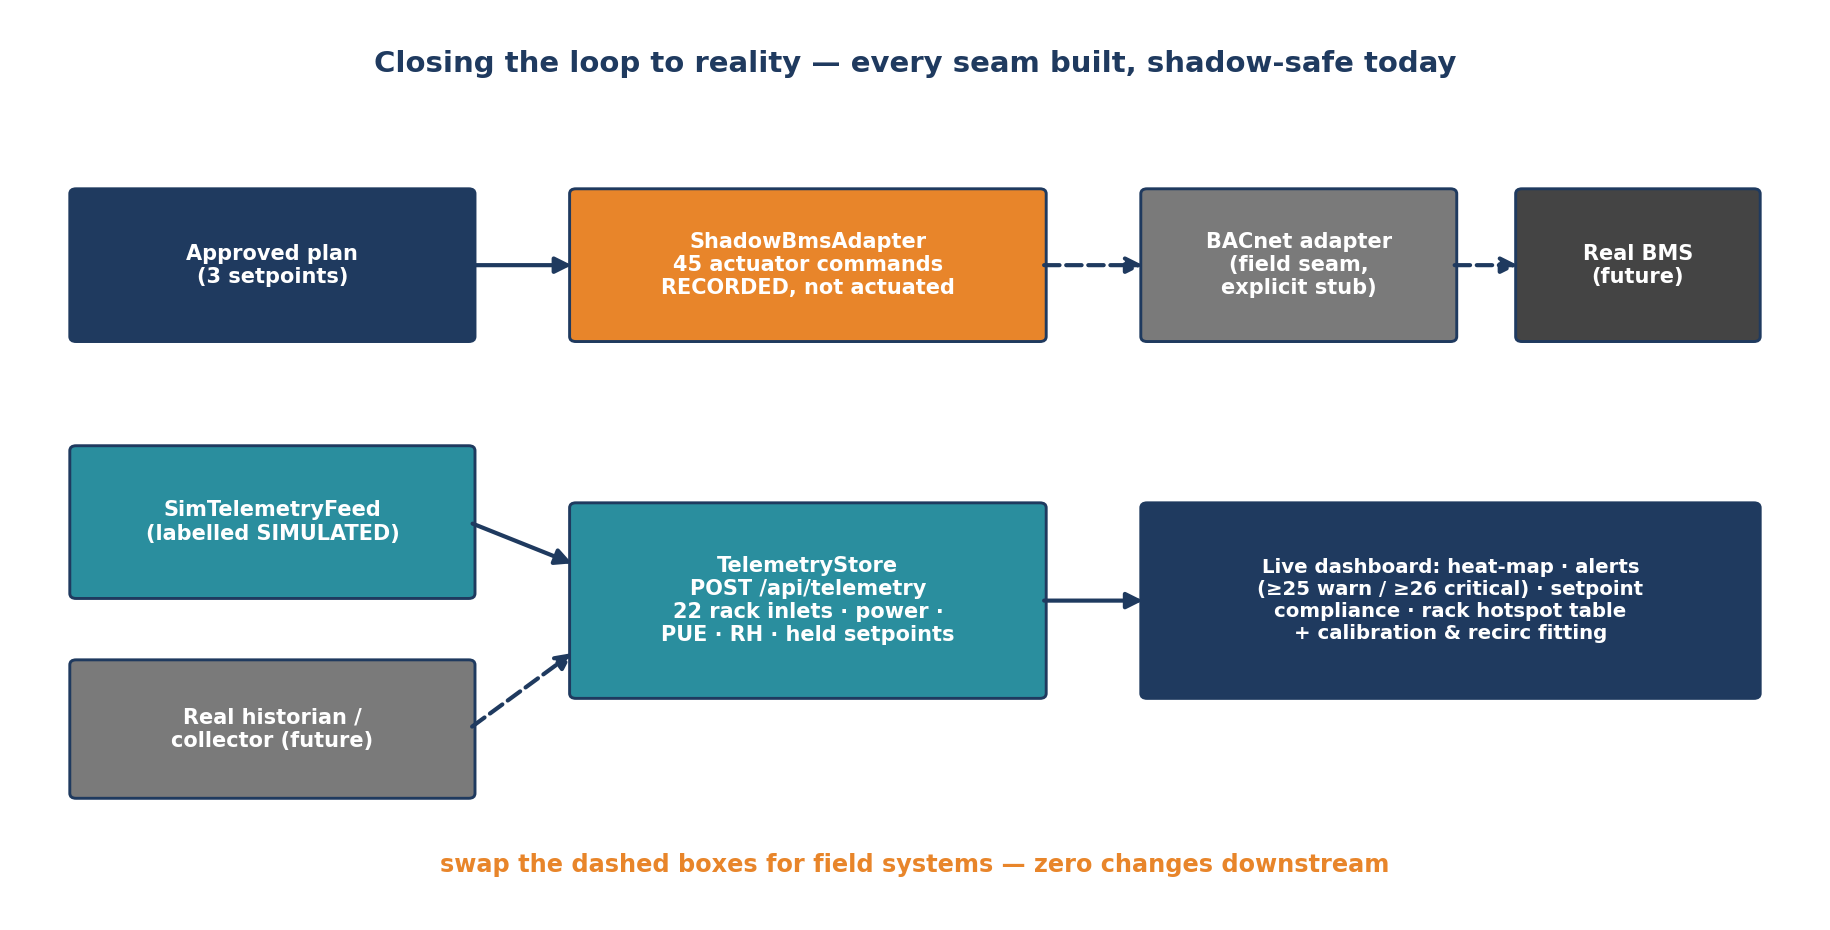
\includegraphics[width=\linewidth]{figures/figE_dataflow.png}\caption{Closing the loop. An approved plan becomes 45 recorded commands; measured outcomes flow back to update the twin's bias and uncertainty (and, slowly, its physics). The dashed boxes are the only parts not yet connected to a real building.}\label{fig:dataflow}\end{figure}

\subsection{Step one: correct the steady drift (bias)}

If the twin always guesses the inlet air is, say, a fifth of a degree cooler than it really turns out to be, that is not random noise --- it is a consistent lean, like a bathroom scale that always reads two pounds light. The cure is to measure the average miss and subtract it next time.

\begin{equation}\label{eq:bias}
b = \operatorname{mean}\big(\text{winsorized prediction errors}\big).
\end{equation}
\plainwords{$b$ is the twin's typical drift --- the average amount by which its prediction missed reality across the week. We ``winsorize'' the errors first, which just means we clip a few freak outliers back to a sane range so a single weird fifteen-minute step can't yank the average around. From now on the twin shifts its forecast by $b$ to cancel that lean.}

\subsection{Step two: know how much to trust yourself (the fading floor)}

Correcting the average drift is only half the story. The twin also has to be honest about how \emph{spread out} its mistakes are --- its uncertainty $\sigma$. This number matters enormously, because the safety gate of Net 1 turns $\sigma$ directly into a margin below the $26\,^\circ$C cap: the less the twin trusts itself, the more thermal headroom it leaves on the table. Here lies a trap. After a single deployed week, you have almost no evidence about how variable the errors are. If the twin naively measured the spread from one week, it might happen to see a calm week and declare itself supremely confident --- exactly when it has earned no such right.

\begin{analogy}
Imagine a new weather forecaster who gets one sunny day right and announces, ``I never miss.'' You would not bet your wedding on her yet. You want her to stay cautious until she has a track record. The fading floor enforces exactly this caution.
\end{analogy}

\begin{equation}\label{eq:fadingfloor}
\sigma_{\text{floor}} = \max\!\left(s,\ \frac{\sigma_{\text{prior}}}{n}\right).
\end{equation}
\plainwords{$\sigma_{\text{floor}}$ is the smallest uncertainty the twin is allowed to claim. $s$ is the spread it actually measured from the data so far. $\sigma_{\text{prior}}$ is the cautious starting guess we hard-code before any data exists ($1.0\,^\circ$C for inlet). $n$ is how many weeks of evidence we have. Early on, $n$ is tiny, so $\sigma_{\text{prior}}/n$ is large and \emph{wins} the $\max$ --- the twin is forced to stay humble. As the weeks pile up, that term fades away (it is divided by an ever-larger $n$), and the twin is allowed to trust the data it has actually collected. Hence ``fading floor'': a humility floor that lowers itself only as evidence accumulates.}

\subsection{Step three: blend caution with evidence (empirical Bayes)}

The fading floor sets a \emph{lower bound} on uncertainty; the next step decides the actual number the twin will carry forward. Rather than swing between ``trust the prior'' and ``trust the data,'' we blend them. The trick is to treat our cautious prior guess as if it were one extra week of (imaginary) experience.

\begin{equation}\label{eq:ebblend}
\sigma_{\text{post}} = \sqrt{\frac{n\,s^{2} + \sigma_{\text{prior}}^{2}}{n+1}}.
\end{equation}
\plainwords{$\sigma_{\text{post}}$ is the twin's final, settled uncertainty after the update --- the number the safety margin is built from. Read the fraction as a weighted average of two ideas: the $n$ real weeks of measured spread ($s^2$) and one ``pseudo-week'' speaking for the cautious prior ($\sigma_{\text{prior}}^2$). The ``$+1$'' in the bottom is that pseudo-week getting its vote. So with $n=1$ real week, the prior still counts for half; only as $n$ grows does the evidence outvote it. This is why one lucky, calm week can't make the twin over-confident --- the prior always gets to keep one seat at the table.}

\subsection{Step four: occasionally fix the engine, not just the dials (physics recalibration)}

Bias and uncertainty are gentle, week-to-week tweaks --- adjusting the simulator's instruments. But sometimes the drift on \emph{energy} doesn't go away: it persists week after week, a sign that something structural is off, not just noisy. If the energy prediction stays biased for at least four weeks, the twin does something more invasive: it nudges its own internal physics --- specifically the assumed efficiency of the cooling fans.

\begin{equation}\label{eq:phi}
\phi = \operatorname{clip}\!\left(\frac{1}{1+b},\ 0.85,\ 1.15\right).
\end{equation}
\plainwords{$\phi$ is a correction factor multiplied into the model's fan-efficiency. If the twin has been consistently over-predicting energy, the bias $b$ is positive, $1/(1+b)$ is a little below $1$, and $\phi$ shrinks the modelled power slightly to match reality (and vice versa). The \texttt{clip} is the crucial guardrail: $\phi$ is never allowed outside the band $[0.85,\,1.15]$ --- a hard $\pm 15\%$ limit. We never let a few surprising weeks rewrite the building's physics by more than a sliver, because a runaway ``correction'' could break the very predictions the safety gate depends on.}

\begin{keyidea}
Three nested corrections, from gentlest to boldest: cancel the steady drift ($b$), honestly track how much to trust yourself ($\sigma_{\text{post}}$, floored by humility early), and only as a last resort --- and only by a capped $\pm 15\%$ --- adjust the model's physics itself.
\end{keyidea}

\section{Did it work?}
\label{sec:results}

\begin{keyidea}
Over six consecutive deployed weeks the twin's predictions got sharper, the energy savings grew --- but only as fast as proven safety allowed --- and the hard $26\,^\circ$C line was never once crossed.
\end{keyidea}

We deployed the framework for six consecutive weeks, from 8 November to 13 December 2024. The story that emerged has three threads, and the order matters: the twin first earned \emph{accuracy}, that accuracy bought \emph{confidence}, and only confidence was allowed to release \emph{savings} --- never the other way around.

\subsection{Accuracy: the twin learned to predict reality}

Recall the thermostat dilemma: a nervous operator over-cools because they cannot trust any prediction of how hot things will get. The only way out is a forecast you can believe. In week one, the twin's prediction of the building's weekly cooling energy was off by $1.33\%$. With the calibration loop of Section~\ref{sec:learning} doing its quiet work, that error fell week by week: $1.33\%$, then $0.86\%$, then $0.21\%$, $0.19\%$, $0.08\%$, and $0.10\%$ --- roughly a tenfold improvement, settling around a tenth of a percent. Figure~\ref{fig:accuracy} shows the curve. After a handful of weeks, the simulator was flying like the real plane.

\begin{figure}[t]\centering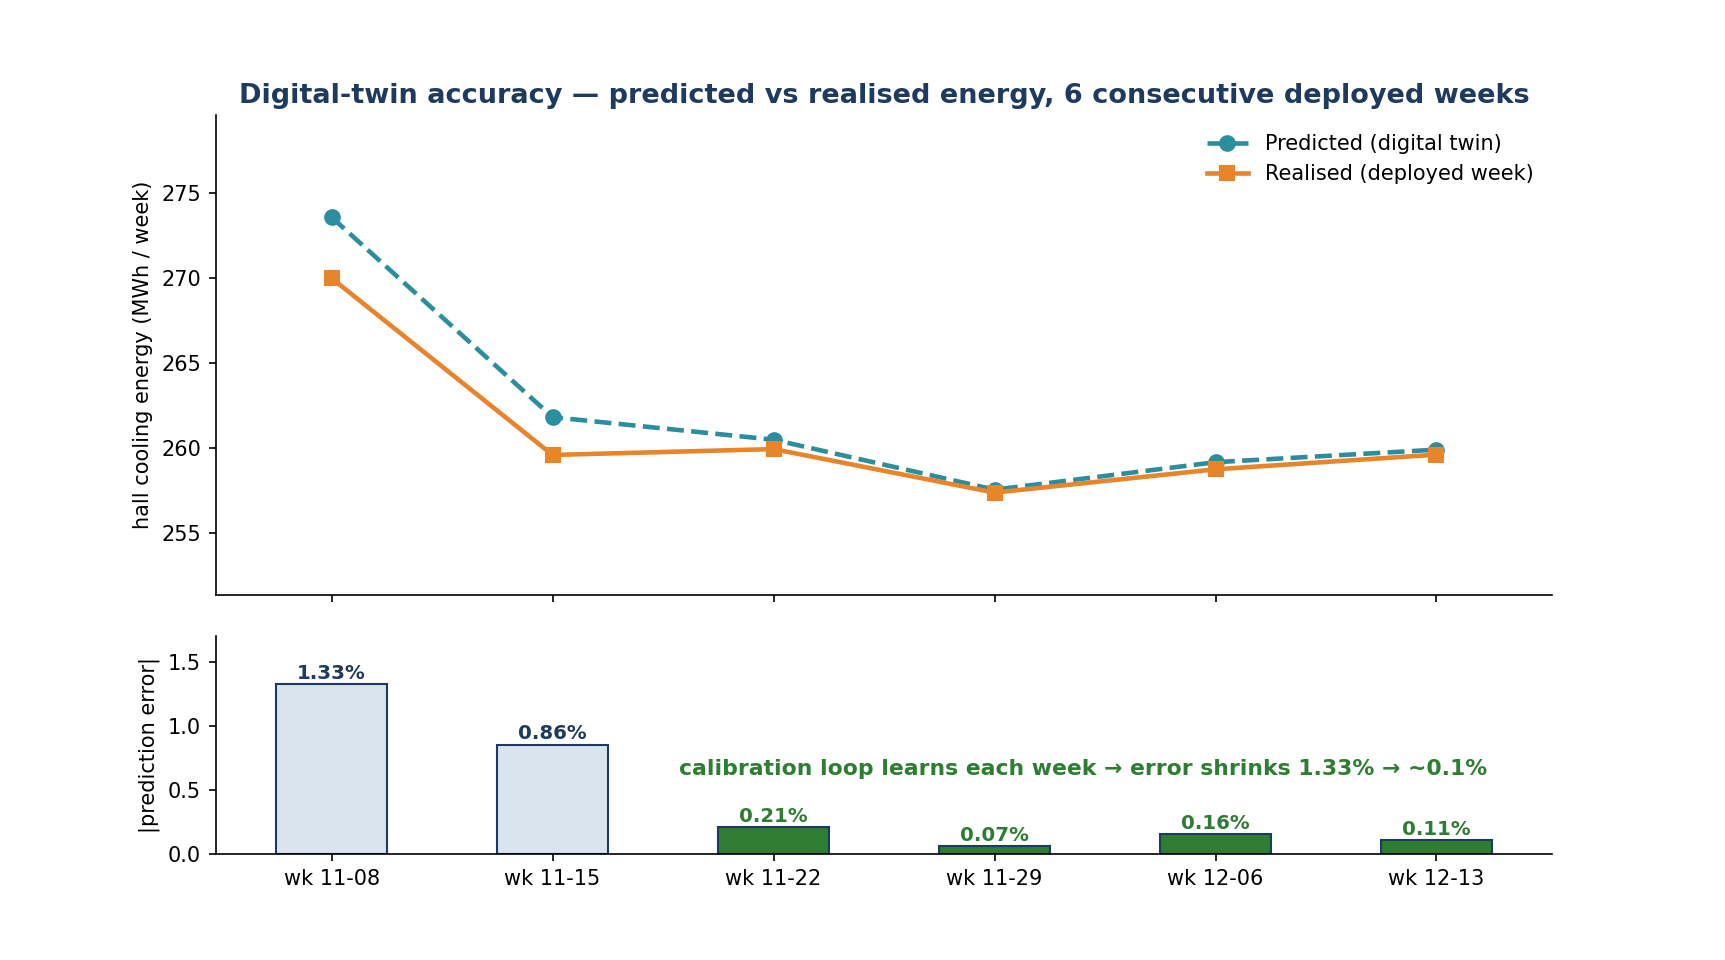
\includegraphics[width=\linewidth]{figures/figA_accuracy.png}\caption{The twin learns to predict reality: weekly-energy prediction error shrinks from 1.33\% to about 0.1\% over six weeks as the calibration loop corrects its bias.}\label{fig:accuracy}\end{figure}

\subsection{Savings: released only as fast as confidence was earned}

Here is the discipline that distinguishes this framework from a reckless one. The twin did not grab the full energy saving on day one. The safety gate spends thermal headroom only when the twin's uncertainty $\sigma$ has shrunk enough to prove that headroom is real. So savings ramped in lock-step with confidence: $0\%$ in the cautious first week, then $3.20\%$, $3.23\%$, $3.60\%$, $3.64\%$, and $3.63\%$. Figure~\ref{fig:savings} shows savings climbing as $\sigma$ falls. The plan settles at roughly a $3.6\%$ reduction in cooling energy against the as-operated baseline, running the hall at a PUE of about $1.19$.

\begin{figure}[t]\centering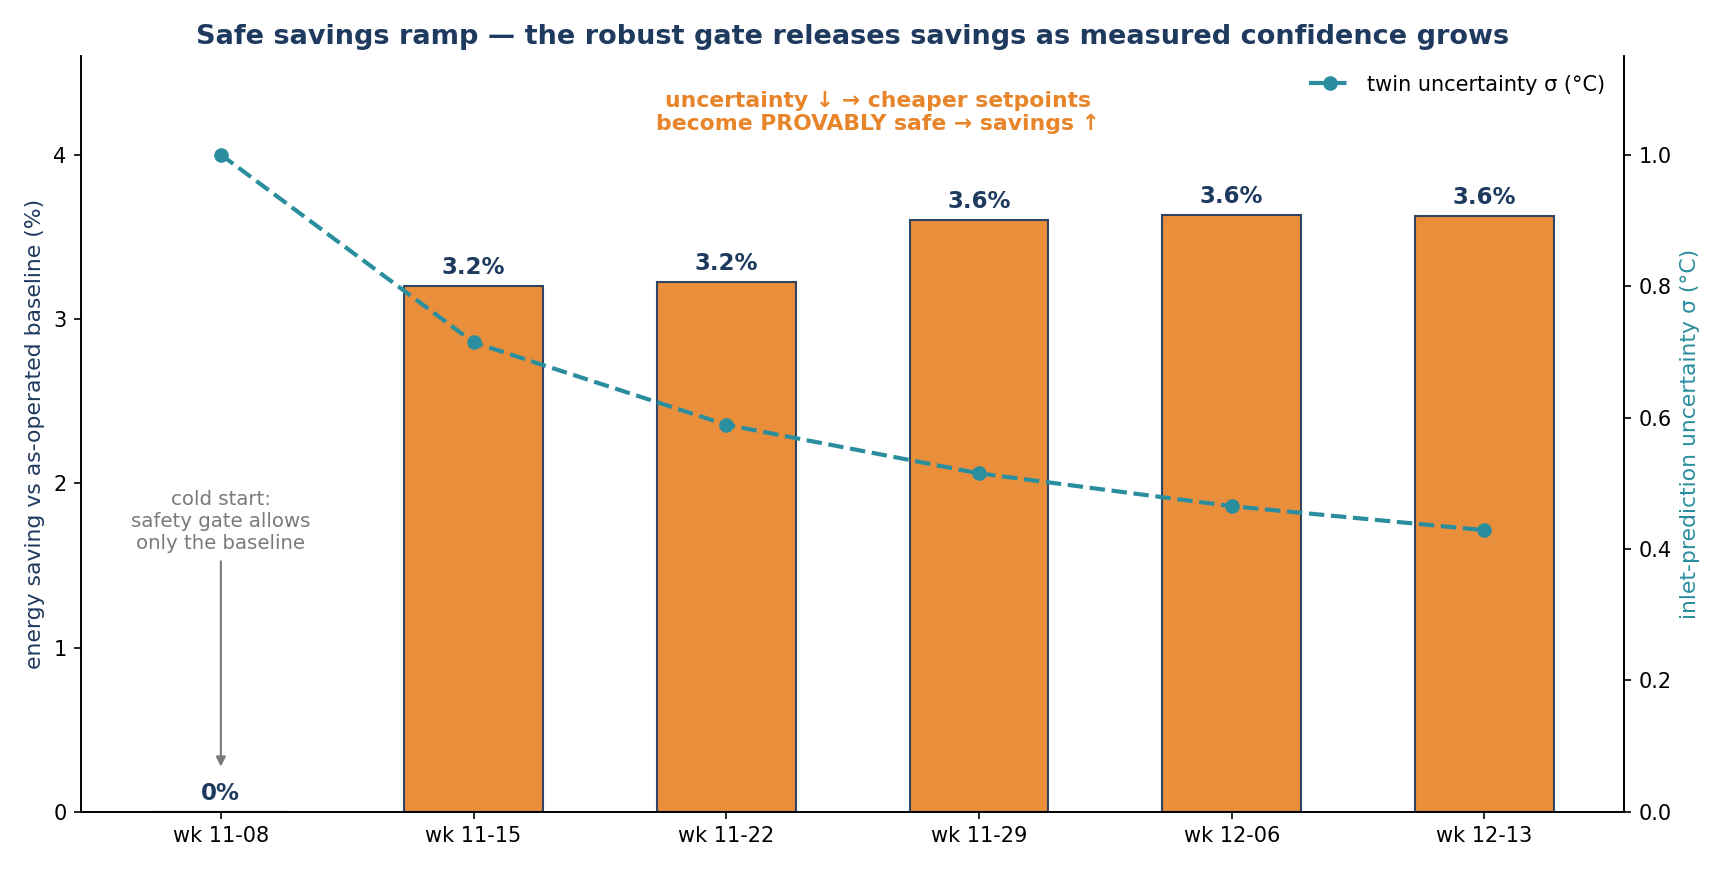
\includegraphics[width=\linewidth]{figures/figB_savings.png}\caption{Savings released by earned confidence: energy saving climbs from 0\% to about 3.6\% as the twin's uncertainty $\sigma$ falls --- the safety gate only spends thermal headroom it has proven is safe.}\label{fig:savings}\end{figure}

That the savings are real and worth chasing is confirmed by the well-posedness sweep we met in Figure~\ref{fig:wellposed}: airflow alone moves the hall's cooling energy by $15.5\%$, chilled-water temperature (CHWST) by $3.4\%$, and supply-air temperature ($T_{\text{supply}}$) by about $0.5\%$. The catch --- and the whole reason a hard-constrained search is necessary --- is that the cheapest setting (the lowest airflow) is also the \emph{hottest}. Saving energy and staying safe pull in opposite directions, so every dollar of saving must be wrung out under the watch of the safety cap.

\subsection{Safety: the line was never crossed}

This is the thread that was never allowed to break. As the twin grew bolder and ran the hall warmer to save energy, the realized peak inlet temperature climbed --- from $23.37\,^\circ$C in the cautious first week up to $25.60\,^\circ$C by the end. But it never reached the $26\,^\circ$C cap. The closest call left a worst-case margin of $0.40\,^\circ$C, and across all six deployed weeks there were \emph{zero} violations. Figure~\ref{fig:saferecord} plots this: a line rising confidently toward the cap, and stopping short every single time. The three-layer safety net --- the $k\sigma$ pre-tightened search cap, the robust stress-test ensemble, and the deploy backstop --- did its job.

\begin{figure}[t]\centering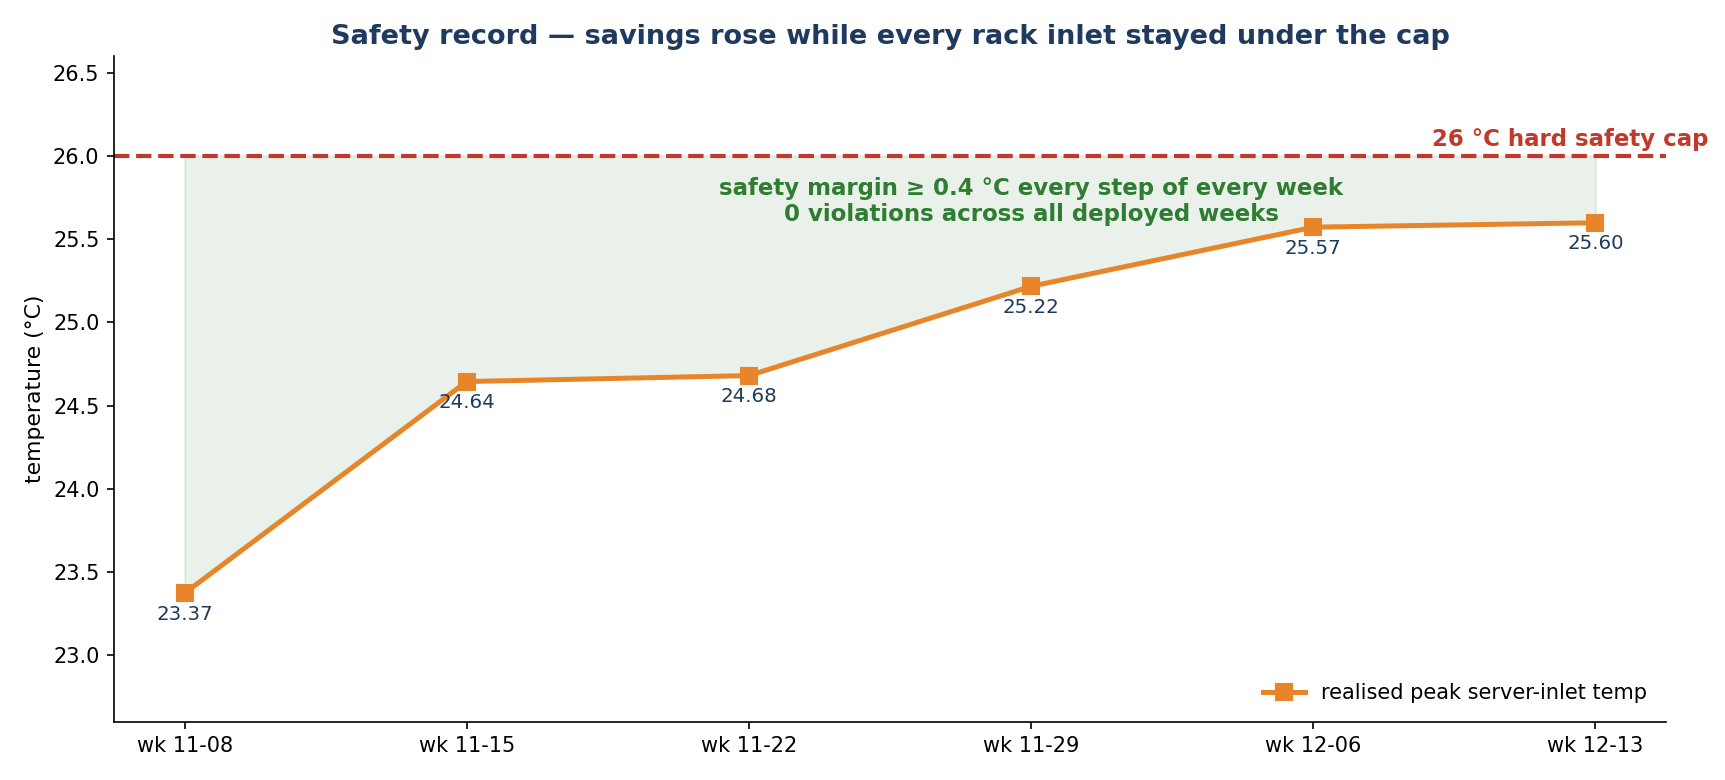
\includegraphics[width=0.85\linewidth]{figures/figC_safety.png}\caption{The line is never crossed: realized peak inlet rises toward, but never reaches, the 26\,$^\circ$C cap (worst case 25.60\,$^\circ$C; zero violations in every deployed week).}\label{fig:saferecord}\end{figure}

After seven weeks of calibration, the twin's settled internal state tells the same story of earned trust: an inlet bias of about $0.18\,^\circ$C, a fading-floor inlet uncertainty of about $0.14\,^\circ$C, a posterior $\sigma_{\text{post}}$ of about $0.36\,^\circ$C, and an energy bias near $515$\,kWh --- roughly $0.2\%$. These are small, stable numbers: the marks of a model that knows what it knows.

\subsection{What the operator sees}

All of this collapses, for the human in the loop, into a single screen. Figure~\ref{fig:webapp} shows the operator's dashboard: the three chosen dials ($T_{\text{supply}}$, airflow, CHWST), the twin's predicted energy and safety numbers set against the current baseline, and the resulting percentage saving --- the entire weekly decision at a glance, with the safety margin to the $26\,^\circ$C cap always in view.

\begin{figure}[t]\centering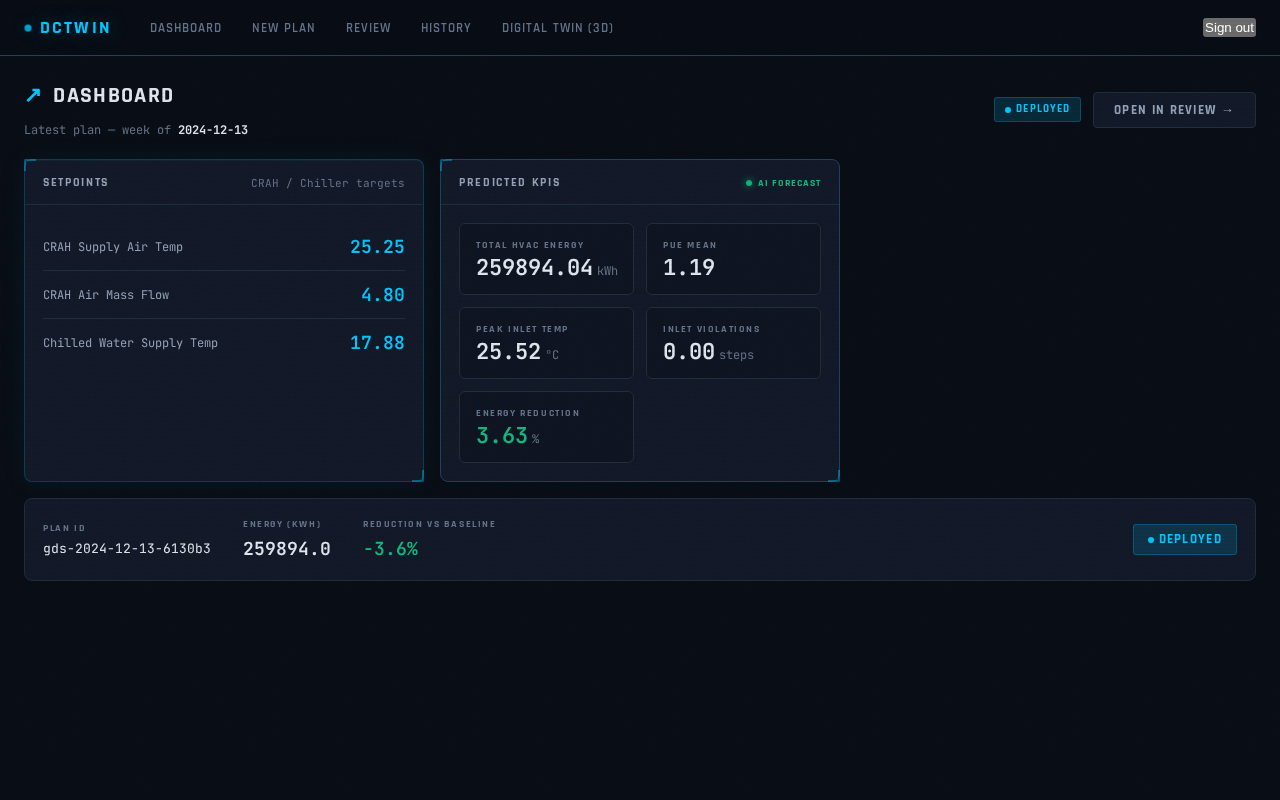
\includegraphics[width=0.9\linewidth]{figures/shot_dashboard.png}\caption{The operator's screen: the chosen dials, the predicted energy and safety numbers against the current baseline, and the percentage saving --- the whole decision at a glance.}\label{fig:webapp}\end{figure}

\section{Honest limits, and the bigger picture}

We have just walked through a system that, every week, quietly tries on dozens of risky cooling strategies inside a simulation, throws away every one that would ever overheat a server, and hands its human operators the single cheapest plan that survives. Over six consecutive weeks the twin learned the building so well that its energy forecast drifted from a $1.33\%$ miss down to roughly a tenth of one percent; it found cooling savings near $3.6\%$ versus how the room was actually being run; and it never once let an inlet cross the $26\,^\circ$C line. Those are real numbers, measured end to end. Before we celebrate, we owe you the fine print.

\subsection{What ``deployed'' really means here}

\begin{keyidea}
Every result in this chapter was produced with the learning loop fully closed and measured --- but the loop was closed around a stand-in for the building, not the building itself.
\end{keyidea}

Three honest caveats. We state them plainly because a safety system that exaggerates its own track record is a contradiction in terms.

\paragraph{Shadow mode.} When the planner approves a weekly plan, it expands the three dials into 45 actuator commands --- and then \emph{records} those commands rather than sending them to any real air handler. Nothing physical moves. This is deliberate: you do not let a new autopilot fly a real plane full of passengers on day one. You let it fly the flight simulator, log every control input it would have made, and check those inputs against what a careful human pilot would have done. Shadow mode is exactly that logbook. The full command path --- search, safety gates, approval, broadcast to 45 actuators --- runs for real; only the final wire to the equipment is left unplugged.

\paragraph{Simulated telemetry.} The ``live'' feed of temperatures and powers that the dashboard displays, and that the calibration step learns from, is a clearly \emph{labelled simulated stream}. It behaves like a real sensor historian would, but it is generated, not measured off a physical probe. We label it as simulated everywhere it appears so that no reader, and no future operator, can mistake it for ground truth from the room.

\paragraph{``Realized'' weeks are a tougher simulation, not the building.} When we report what ``really happened'' after a plan was deployed --- the realized peak inlet rising from $23.37$ to $25.60\,^\circ$C, the savings the gate actually released --- those outcomes come from running the plan on a \emph{perturbed-plant} EnergyPlus simulation: a copy of the building model deliberately made a little worse and a little hotter than the model the planner used to choose the plan. This is the honest way to test a forecast --- judge it against a world that is not quite the world it expected --- but it is still a simulation standing in for the real hall. The gap that remains is a \emph{field connection}: a BACnet adapter to actually carry the 45 commands to the equipment, and a real sensor historian to feed back what truly happened.

So here is the precise, unembellished claim. The dual-loop framework --- search under a hard safety cap, soft penalties for everything else, uncertainty that shrinks the safe operating margin only as evidence accumulates, and recalibration after each week --- is \emph{structurally proven and quantitatively measured} end to end. It is \emph{not yet field-proven}. Bridging that last gap is engineering and access, not a new idea; the architecture is built to accept it without redesign.

\subsection{Why we trust the shape of the result anyway}

Even a stand-in building tells you something real if it is honest about physics, and EnergyPlus is. Two findings travel beyond the simulation. First, the well-posedness sweep showed that, of the three dials, airflow moves hall cooling energy by about $15.5\%$, chilled-water temperature by $3.4\%$, and supply-air temperature by only about $0.5\%$ --- and that the cheapest setting (the lowest airflow) is also the hottest. That single fact is the whole reason a hard-constrained search has to exist: the direction of ``save money'' points straight at the direction of ``overheat a server,'' so something must hold the safety line while the optimizer pushes on cost. Second, the savings did not arrive all at once; the deployment gate released them as $0\%$, then about $3.2\%$, then about $3.6\%$, growing only as the twin's forecast error fell and its confidence earned the right to be bolder. A system that grabbed the full saving on week one would be a system that hadn't yet learned to be afraid of the right things.

\subsection{The bigger picture: a recipe for letting AI optimize safely}

Now step back from cooling towers and chilled water. The thermostat dilemma --- over-cool to feel safe and you burn money; under-cool to save money and you risk the hardware --- is just one face of a problem that shows up everywhere we ask software to optimize something that also carries danger. Dose a patient with enough drug to work but never enough to harm. Trade aggressively for return but never past a loss you cannot survive. Run a power grid hot enough to be cheap but never past a blackout. In every one of these, ``make it cheaper / faster / better'' sits right next to ``and please don't cause a catastrophe.''

DCTwin is a worked example of a general discipline for exactly that situation, and the discipline is simple enough to say in four moves:

\begin{enumerate}
  \item \textbf{Make the dangerous thing a hard wall, not a preference.} The $26\,^\circ$C inlet cap is never traded against money. A plan that crosses it scores infinitely badly and is thrown out --- it cannot be ``bought back'' by being cheap. Catastrophic outcomes should be constraints, not line items.
  \item \textbf{Optimize everything else softly.} Comfort drift in humidity and zone temperature gets a gentle penalty, not a wall. You bend on what's negotiable so you can be rigid on what isn't.
  \item \textbf{Quantify your uncertainty, and let it cost you margin.} The twin doesn't pretend to know the inlet temperature exactly; it carries an uncertainty $\sigma$ and pulls its own safety line inward by that amount. When it knows little, it acts timidly. Honest doubt buys real safety.
  \item \textbf{Earn boldness from real measurements.} Only after the world confirms the forecast does the system tighten its margin and release more savings. Trust is a balance that has to be filled by evidence before it can be spent.
\end{enumerate}

\begin{keyidea}
To let an AI optimize something that can also be dangerous: wall off the catastrophe as a hard constraint, optimize the rest softly, price your own uncertainty into your safety margin, and grow bolder only as fast as real-world evidence lets you.
\end{keyidea}

\begin{analogy}
It is the difference between a reckless driver and a good one learning a new road at night. The reckless driver floors it and hopes. The good one starts slow, leaves extra room because they can't see far, and speeds up only as the headlights --- and a few safe miles --- reveal that the road is exactly where they thought it was. DCTwin is built to drive the second way.
\end{analogy}

The honest limits and the bigger picture are really the same point seen from two sides. We did not let the system touch the real building yet --- precisely because the whole philosophy is to earn trust before spending it. The loop is proven, the physics is faithful, the savings are real in simulation, and the safety record is spotless across every week we ran. What remains is a wire and a sensor feed, not a leap of faith. When that field connection is made, the framework is ready to start the same patient, measurable, trust-earning climb on a real hall --- and, we hope, on the many other systems where the cheapest path and the safest path are not the same, and somebody has to hold both at once.

\section*{Key takeaways}

\begin{keyidea}
\begin{itemize}
  \item \textbf{One dilemma, two anchors.} Cooling a data center is the thermostat dilemma --- over-cool and you burn money, under-cool and you risk the hardware --- and DCTwin escapes it by rehearsing every risky move in a ``flight simulator'' (a full-physics digital twin running EnergyPlus) before touching the real plant.
  \item \textbf{Three dials, one hard line.} Just three weekly setpoints --- supply-air temperature $T_{\text{supply}}$, CRAH airflow, and chilled-water temperature CHWST --- are broadcast to 45 actuators, all under one non-negotiable rule: every server inlet stays $\le 26\,^\circ$C at every fifteen-minute step.
  \item \textbf{Search the safe region only.} A coarse-to-fine beam search ($5\times5\times5 = 125$ candidates, refined over three halving levels) minimises a single score $J$ --- mostly weekly energy $E_{\text{hvac}}$ plus soft comfort penalties --- while any unsafe candidate is disqualified with $J = +\infty$.
  \item \textbf{Safety is layered, not assumed.} A $k\sigma$ margin baked into the search ($k=1$), a CVaR stress-test ensemble against a worse-than-expected plant, and a zero-tolerance deploy backstop together kept the realized peak inlet at $25.60\,^\circ$C --- with zero violations across six weeks.
  \item \textbf{Confidence is earned, then spent.} The twin's energy error fell from $1.33\%$ to about $0.10\%$, and only as its uncertainty $\sigma$ shrank did the gate release savings --- $0\% \to 3.6\%$ against the as-operated baseline, at a PUE of about $1.19$.
  \item \textbf{Proven, not yet field-proven.} The whole loop is structurally proven and measured, but it runs in shadow mode: commands are recorded not actuated, telemetry is a labelled simulated feed, and ``realized'' weeks come from a perturbed-plant simulation until a real field connection exists.
\end{itemize}
\end{keyidea}

\section*{A mini-glossary}

\begin{description}
  \item[Digital twin] A faithful computer model of the real building --- the ``flight simulator'' --- used to rehearse cooling decisions safely before any of them touch the physical hall.
  \item[EnergyPlus / oracle] EnergyPlus (version 9.5, run in Docker) is the industry-standard building-physics engine inside the twin. Because it is consulted on every candidate plan and judges it, we call it the \emph{oracle}: it plays a full week forward in fifteen-minute steps and reports energy and peak inlet temperature.
  \item[SAT / CHWST] SAT is the supply-air temperature $T_{\text{supply}}$ ($20$--$26\,^\circ$C), how cold the air blown into the room is. CHWST is the chilled-water supply temperature ($13$--$19\,^\circ$C), how cold the water the plant chills to make that air.
  \item[Inlet cap] The hard $26\,^\circ$C ceiling on $T_{\text{inlet}}$, the temperature of the air each server actually breathes. It must hold at every fifteen-minute step; it is a constraint, never a trade-off.
  \item[Beam search] A coarse-to-fine optimisation: lay a $5\times5\times5$ grid of candidate settings, keep the best five (the ``beam''), refine around them with the grid spacing halved each level, and stop when the score barely improves.
  \item[PUE] Power Usage Effectiveness --- total facility power divided by computing (IT) power, averaged over time. A PUE of $1$ is the unreachable ideal; DCTwin's plan runs at about $1.19$.
  \item[$\sigma$ / uncertainty] The twin's honest estimate of how far off its inlet prediction might be. It starts cautious ($1.0\,^\circ$C at cold start), shrinks as the twin proves itself, and directly sets the safety margin below the cap.
  \item[CVaR] Conditional Value at Risk --- the average of the worst outcomes (here, the worst $20\%$, at $\alpha = 0.8$). It grades a plan by its bad days rather than its average day, so robustness, not luck, wins.
  \item[Shadow mode] The current deployment state: the 45 commands are computed and recorded but never physically actuated, the live telemetry is a labelled simulated feed, and ``realized'' weeks come from a perturbed-plant simulation --- proven end to end, but not yet field-proven.
\end{description}\end{document}
